%----------------------------------------------------------------------------------------
%	SOLUTION 2
%----------------------------------------------------------------------------------------
\subsection*{Solution 2}
%----------------------------------------------------------------------------------------
%	SOLUTION 2
%----------------------------------------------------------------------------------------
\paragraph{Summary:} Here I have used Tensorflow to build a feed forward neural network. The network is learned using stochastic gradient descent (SGD) algorithm for weight update using a mini batch size of $32$. SGD is used without momentum and with a learning rate of $0.01$. I have also converted labels to \textit{one-hot} representation to use \textit{categorical crossentropy} as the loss for Tensorflow model. The input features are scaled to $[0, 1]$ as I have seen this improves the performance of the neural network a lot.
\paragraph{Convergence criteria used:} I have declared convergence if in $3$ consecutive epochs the decrease of loss is less than $0.001$ or loss increases for $3$ consecutive epochs. The maximum number of epochs has a limit of $100$ though I have never seen hitting this limit before convergence is achieved.
\paragraph{Results:} Fig.~\ref{fig:q2_loss_acc} shows the cumulative loss and accuracy with increasing nuber of epochs.
%%%%%%%%%%%%%%%%%%%%%%% SGD LOSS + ACCURACY %%%%%%%%%%%%%%%%%%%%%
\begin{figure}[!h]
	\centering
	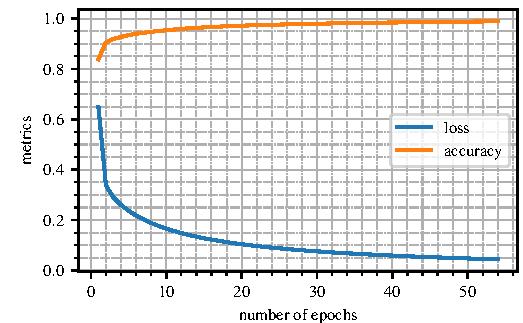
\includegraphics[scale=1.0,trim={0cm 0cm 0cm 0cm},clip]{./code/generatedPlots/q2_loss_acc.pdf}
	\caption{Q2: SGD cumulative training loss and accuracy with different epochs: Feedforward neural net}
	\label{fig:q2_loss_acc}
\end{figure}
From Fig.~\ref{fig:q2_loss_acc}, we can see that as we increase the number of epochs, the network learns better and thus the loss decreases monotonically and the accuracy increases. Table~\ref{tbl:q2_sgd_loss_acc} shows the training loss and accuracy after convergence and test loss and accuracy.
%%%%%%%%%%%%%%%%%%%%%%%%%% TRAIN+TEST %%%%%%%%%%%%%%%%%%%%%%%%%%%%%%%%%%%
\begin{table}[ht]
	\centering
	\caption{Q2: Train (after convergence) and test loss and accuracy}
	\begin{tabular}[t]{ccc} 
		\hline
		 			& Loss & Accuracy(\%)\\ [0.5ex] 
		\hline
		Train 	& $0.044$ 	& $98.88$\\
		Test 	& $0.077$ 	& $97.60$\\[1ex]
		\hline
	\end{tabular}
	\label{tbl:q2_sgd_loss_acc}
\end{table}